\documentclass[]{book}
\usepackage{lmodern}
\usepackage{amssymb,amsmath}
\usepackage{ifxetex,ifluatex}
\usepackage{fixltx2e} % provides \textsubscript
\ifnum 0\ifxetex 1\fi\ifluatex 1\fi=0 % if pdftex
  \usepackage[T1]{fontenc}
  \usepackage[utf8]{inputenc}
\else % if luatex or xelatex
  \ifxetex
    \usepackage{mathspec}
  \else
    \usepackage{fontspec}
  \fi
  \defaultfontfeatures{Ligatures=TeX,Scale=MatchLowercase}
\fi
% use upquote if available, for straight quotes in verbatim environments
\IfFileExists{upquote.sty}{\usepackage{upquote}}{}
% use microtype if available
\IfFileExists{microtype.sty}{%
\usepackage{microtype}
\UseMicrotypeSet[protrusion]{basicmath} % disable protrusion for tt fonts
}{}
\usepackage[margin=1in]{geometry}
\usepackage{hyperref}
\hypersetup{unicode=true,
            pdftitle={Curso de R para meteorologia IAG/USP},
            pdfauthor={Sergio Ibarra-Espinosa, Amanda Rehbein, Daniel Schuch, e possivelmente outros (u r invited to collaborate)},
            pdfborder={0 0 0},
            breaklinks=true}
\urlstyle{same}  % don't use monospace font for urls
\usepackage{natbib}
\bibliographystyle{apalike}
\usepackage{color}
\usepackage{fancyvrb}
\newcommand{\VerbBar}{|}
\newcommand{\VERB}{\Verb[commandchars=\\\{\}]}
\DefineVerbatimEnvironment{Highlighting}{Verbatim}{commandchars=\\\{\}}
% Add ',fontsize=\small' for more characters per line
\usepackage{framed}
\definecolor{shadecolor}{RGB}{248,248,248}
\newenvironment{Shaded}{\begin{snugshade}}{\end{snugshade}}
\newcommand{\KeywordTok}[1]{\textcolor[rgb]{0.13,0.29,0.53}{\textbf{#1}}}
\newcommand{\DataTypeTok}[1]{\textcolor[rgb]{0.13,0.29,0.53}{#1}}
\newcommand{\DecValTok}[1]{\textcolor[rgb]{0.00,0.00,0.81}{#1}}
\newcommand{\BaseNTok}[1]{\textcolor[rgb]{0.00,0.00,0.81}{#1}}
\newcommand{\FloatTok}[1]{\textcolor[rgb]{0.00,0.00,0.81}{#1}}
\newcommand{\ConstantTok}[1]{\textcolor[rgb]{0.00,0.00,0.00}{#1}}
\newcommand{\CharTok}[1]{\textcolor[rgb]{0.31,0.60,0.02}{#1}}
\newcommand{\SpecialCharTok}[1]{\textcolor[rgb]{0.00,0.00,0.00}{#1}}
\newcommand{\StringTok}[1]{\textcolor[rgb]{0.31,0.60,0.02}{#1}}
\newcommand{\VerbatimStringTok}[1]{\textcolor[rgb]{0.31,0.60,0.02}{#1}}
\newcommand{\SpecialStringTok}[1]{\textcolor[rgb]{0.31,0.60,0.02}{#1}}
\newcommand{\ImportTok}[1]{#1}
\newcommand{\CommentTok}[1]{\textcolor[rgb]{0.56,0.35,0.01}{\textit{#1}}}
\newcommand{\DocumentationTok}[1]{\textcolor[rgb]{0.56,0.35,0.01}{\textbf{\textit{#1}}}}
\newcommand{\AnnotationTok}[1]{\textcolor[rgb]{0.56,0.35,0.01}{\textbf{\textit{#1}}}}
\newcommand{\CommentVarTok}[1]{\textcolor[rgb]{0.56,0.35,0.01}{\textbf{\textit{#1}}}}
\newcommand{\OtherTok}[1]{\textcolor[rgb]{0.56,0.35,0.01}{#1}}
\newcommand{\FunctionTok}[1]{\textcolor[rgb]{0.00,0.00,0.00}{#1}}
\newcommand{\VariableTok}[1]{\textcolor[rgb]{0.00,0.00,0.00}{#1}}
\newcommand{\ControlFlowTok}[1]{\textcolor[rgb]{0.13,0.29,0.53}{\textbf{#1}}}
\newcommand{\OperatorTok}[1]{\textcolor[rgb]{0.81,0.36,0.00}{\textbf{#1}}}
\newcommand{\BuiltInTok}[1]{#1}
\newcommand{\ExtensionTok}[1]{#1}
\newcommand{\PreprocessorTok}[1]{\textcolor[rgb]{0.56,0.35,0.01}{\textit{#1}}}
\newcommand{\AttributeTok}[1]{\textcolor[rgb]{0.77,0.63,0.00}{#1}}
\newcommand{\RegionMarkerTok}[1]{#1}
\newcommand{\InformationTok}[1]{\textcolor[rgb]{0.56,0.35,0.01}{\textbf{\textit{#1}}}}
\newcommand{\WarningTok}[1]{\textcolor[rgb]{0.56,0.35,0.01}{\textbf{\textit{#1}}}}
\newcommand{\AlertTok}[1]{\textcolor[rgb]{0.94,0.16,0.16}{#1}}
\newcommand{\ErrorTok}[1]{\textcolor[rgb]{0.64,0.00,0.00}{\textbf{#1}}}
\newcommand{\NormalTok}[1]{#1}
\usepackage{longtable,booktabs}
\usepackage{graphicx,grffile}
\makeatletter
\def\maxwidth{\ifdim\Gin@nat@width>\linewidth\linewidth\else\Gin@nat@width\fi}
\def\maxheight{\ifdim\Gin@nat@height>\textheight\textheight\else\Gin@nat@height\fi}
\makeatother
% Scale images if necessary, so that they will not overflow the page
% margins by default, and it is still possible to overwrite the defaults
% using explicit options in \includegraphics[width, height, ...]{}
\setkeys{Gin}{width=\maxwidth,height=\maxheight,keepaspectratio}
\IfFileExists{parskip.sty}{%
\usepackage{parskip}
}{% else
\setlength{\parindent}{0pt}
\setlength{\parskip}{6pt plus 2pt minus 1pt}
}
\setlength{\emergencystretch}{3em}  % prevent overfull lines
\providecommand{\tightlist}{%
  \setlength{\itemsep}{0pt}\setlength{\parskip}{0pt}}
\setcounter{secnumdepth}{5}
% Redefines (sub)paragraphs to behave more like sections
\ifx\paragraph\undefined\else
\let\oldparagraph\paragraph
\renewcommand{\paragraph}[1]{\oldparagraph{#1}\mbox{}}
\fi
\ifx\subparagraph\undefined\else
\let\oldsubparagraph\subparagraph
\renewcommand{\subparagraph}[1]{\oldsubparagraph{#1}\mbox{}}
\fi

%%% Use protect on footnotes to avoid problems with footnotes in titles
\let\rmarkdownfootnote\footnote%
\def\footnote{\protect\rmarkdownfootnote}

%%% Change title format to be more compact
\usepackage{titling}

% Create subtitle command for use in maketitle
\newcommand{\subtitle}[1]{
  \posttitle{
    \begin{center}\large#1\end{center}
    }
}

\setlength{\droptitle}{-2em}
  \title{Curso de R para meteorologia IAG/USP}
  \pretitle{\vspace{\droptitle}\centering\huge}
  \posttitle{\par}
  \author{Sergio Ibarra-Espinosa, Amanda Rehbein, Daniel Schuch, e possivelmente
outros (u r invited to collaborate)}
  \preauthor{\centering\large\emph}
  \postauthor{\par}
  \predate{\centering\large\emph}
  \postdate{\par}
  \date{2018-04-30}

\usepackage{booktabs}
\usepackage{amsthm}
\makeatletter
\def\thm@space@setup{%
  \thm@preskip=8pt plus 2pt minus 4pt
  \thm@postskip=\thm@preskip
}
\makeatother

\usepackage{amsthm}
\newtheorem{theorem}{Theorem}[chapter]
\newtheorem{lemma}{Lemma}[chapter]
\theoremstyle{definition}
\newtheorem{definition}{Definition}[chapter]
\newtheorem{corollary}{Corollary}[chapter]
\newtheorem{proposition}{Proposition}[chapter]
\theoremstyle{definition}
\newtheorem{example}{Example}[chapter]
\theoremstyle{definition}
\newtheorem{exercise}{Exercise}[chapter]
\theoremstyle{remark}
\newtheorem*{remark}{Remark}
\newtheorem*{solution}{Solution}
\begin{document}
\maketitle

{
\setcounter{tocdepth}{1}
\tableofcontents
}
\chapter{Pre-requisitos do sistema}\label{primero}

Em Windows, instale além do R, Rtools
\url{https://cran.r-project.org/bin/windows/Rtools/}

Em MAC instale netcdf e:

\begin{Shaded}
\begin{Highlighting}[]
\ExtensionTok{brew}\NormalTok{ unlink gdal}
\ExtensionTok{brew}\NormalTok{ tap osgeo/osgeo4mac }\KeywordTok{&&} \ExtensionTok{brew}\NormalTok{ tap --repair}
\ExtensionTok{brew}\NormalTok{ install proj}
\ExtensionTok{brew}\NormalTok{ install geos}
\ExtensionTok{brew}\NormalTok{ install udunits}
\ExtensionTok{brew}\NormalTok{ install gdal2 --with-armadillo --with-complete --with-libkml --with-unsupported}
\ExtensionTok{brew}\NormalTok{ link --force gdal2}
\end{Highlighting}
\end{Shaded}

Em Ubuntu:

\begin{Shaded}
\begin{Highlighting}[]
  \ExtensionTok{-}\NormalTok{ sudo add-apt-repository ppa:ubuntugis/ubuntugis-unstable --yes}
  \ExtensionTok{-}\NormalTok{ sudo apt-get --yes --force-yes update -qq}
  \CommentTok{# install tmap dependencies}
  \ExtensionTok{-}\NormalTok{ sudo apt-get install --yes libprotobuf-dev protobuf-compiler libv8-3.14-dev}
  \CommentTok{# install tmap dependencies; for 16.04 libjq-dev this ppa is needed:}
  \ExtensionTok{-}\NormalTok{ sudo add-apt-repository -y ppa:opencpu/jq}
  \ExtensionTok{-}\NormalTok{ sudo apt-get --yes --force-yes update -qq}
  \ExtensionTok{-}\NormalTok{ sudo apt-get install libjq-dev}
  \CommentTok{# units/udunits2 dependency:}
  \ExtensionTok{-}\NormalTok{ sudo apt-get install --yes libudunits2-dev}
  \CommentTok{# sf dependencies:}
  \ExtensionTok{-}\NormalTok{ sudo apt-get install --yes libproj-dev libgeos-dev libgdal-dev libnetcdf-dev  netcdf-bin gdal-bin}
\end{Highlighting}
\end{Shaded}

\section{Pacotes usados neste curso}\label{pacotes-usados-neste-curso}

Para fazer este curso instale os seguintes pacotes como indicado:

\begin{Shaded}
\begin{Highlighting}[]
\KeywordTok{install.packages}\NormalTok{(}\StringTok{"devtools"}\NormalTok{)}
\NormalTok{devtools}\OperatorTok{::}\KeywordTok{install_github}\NormalTok{(}\StringTok{"tidyverse/tidyverse"}\NormalTok{)}
\NormalTok{devtools}\OperatorTok{::}\KeywordTok{install_github}\NormalTok{(}\StringTok{"r-spatial/sf"}\NormalTok{)}
\NormalTok{devtools}\OperatorTok{::}\KeywordTok{install_github}\NormalTok{(}\StringTok{"r-spatial/mapview"}\NormalTok{)}
\NormalTok{devtools}\OperatorTok{::}\KeywordTok{install_github}\NormalTok{(}\StringTok{"r-spatial/stars"}\NormalTok{)}
\KeywordTok{install.packages}\NormalTok{(}\KeywordTok{c}\NormalTok{(}\StringTok{"raster"}\NormalTok{, }\StringTok{"sp"}\NormalTok{, }\StringTok{"rgdal"}\NormalTok{, }\StringTok{"maptools"}\NormalTok{, }\StringTok{"ncdf4"}\NormalTok{))}
\KeywordTok{install.packages}\NormalTok{(}\KeywordTok{c}\NormalTok{(}\StringTok{"cptcity"}\NormalTok{, }\StringTok{"data.table"}\NormalTok{, }\StringTok{"openair"}\NormalTok{))}
\end{Highlighting}
\end{Shaded}

\begin{itemize}
\tightlist
\item
  \href{https://CRAN.R-project.org/package=devtools}{devtools} é um
  pacote para instalar pacotes de diferentes repositórios
\item
  \href{https://github.com/tidyverse}{tidyverse} é o universo de pacotes
  do Hadley Wickham. A instalação tem que ser usando devtools, pois
  precisamos plotar os objetos espacias sf usando
  \href{https://www.isgeomsfinggplot2yet.site/}{geom\_sf}.
\item
  \href{https://github.com/r-spatial/sf}{sf} e
  \href{https://github.com/r-spatial/mapbiew}{mapview},
  \href{https://github.com/r-spatial/stars}{stars}, raster, sp, rgdal e
  maptools são para a parte espacial. Lembrar que os objetos em
  meteorologias são espaço-temporais.
\item
  ncdf4 é um pacote para manipular arquivos NetCDF.
\item
  \href{https://ibarraespinosa.github.io/cptcity/}{cptcity} é um pacote
  que tem 7140 paletas de cores do arquivo web cpt-city
  (\url{http://soliton.vm.bytemark.co.uk/pub/cpt-city/index.html}).
\item
  \href{http://davidcarslaw.github.io/openair/}{openair} é um pacote
  para trabalhar com dados de qualidade do ar e meteorologia.
\end{itemize}

Se faltarem dependencias de sistema, instale elas e instale os pacotes.

\section{Colaborar}\label{colaborar}

A forma preferida de colaboração é com pull-requests em
\url{https://github.com/ibarraespinosa/cursoR/pull/new/master}. Lembre
de aplicar a Guia de Estilo de R de Google
(\url{https://google.github.io/styleguide/Rguide.xml}) ou com o formato
de formatR \url{https://yihui.name/formatr/}. Em poucas palavras, lembre
que seu código vai ser lido por seres humanos. Se quiser tem acesso no
repositório deste curso, me contate. Tem um botão para editar qualquer
página.

\section{Aportar com dados}\label{aportar-com-dados}

Se você tem dados para fazer este curso mais legal, por favor, edite
este aquivo e com pull request, eu vou fazer um merge para poder.

\begin{enumerate}
\def\labelenumi{\arabic{enumi}.}
\item
  NCEP: \url{ftp://nomads.ncdc.noaa.gov/GFS/analysis_only/}
\item
\item
\end{enumerate}

\chapter{Intro}\label{intro}

Este curso é para pos, então vamos ver conteúdo rapidamente e se não da
tempo, este curso esta online no sitio
\url{https://github.com/atmoschem/cursorIAG}.

Eu tento usar
\href{http://stat.ethz.ch/R-manual/R-devel/library/base/html/00Index.html}{BASE}
sempre que posso, e se não da ai vou para outros paradigmas.

Outros pacotes de BASE:
\href{http://stat.ethz.ch/R-manual/R-devel/library/utils/html/00Index.html}{utils},
\href{http://stat.ethz.ch/R-manual/R-devel/library/stats/html/00Index.html}{stats},
\href{http://stat.ethz.ch/R-manual/R-devel/library/datasets/html/00Index.html}{datasets},
\href{http://stat.ethz.ch/R-manual/R-devel/library/graphics/html/00Index.html}{graphics},
\href{https://stat.ethz.ch/R-manual/R-devel/library/grDevices/html/00Index.html}{grDevices},
\href{https://stat.ethz.ch/R-manual/R-devel/library/grid/html/00Index.html}{grid},
\href{https://stat.ethz.ch/R-manual/R-devel/library/methods/html/00Index.html}{methods},
\href{https://stat.ethz.ch/R-manual/R-devel/library/tools/html/00Index.html}{tools},
\href{https://stat.ethz.ch/R-manual/R-devel/library/parallel/html/00Index.html}{parallel},
\href{https://stat.ethz.ch/R-manual/R-devel/library/compiler/html/00Index.html}{compiler},
\href{https://stat.ethz.ch/R-manual/R-devel/library/splines/html/00Index.html}{splines},
\href{https://stat.ethz.ch/R-manual/R-devel/library/tcltk/html/00Index.html}{tcltk}
,
\href{https://stat.ethz.ch/R-manual/R-devel/library/stats4/html/00Index.html}{stats4}.

Veja
\href{https://cran.r-project.org/web/packages/available_packages_by_name.html}{outros}
pacotes.

Este curso esta baseado no livro
\href{https://leanpub.com/rprogramming}{R Programming for Data Science}.

Vamos usar \href{https://www.rstudio.com/}{Rstudio}

\textbf{Dica:}

\begin{itemize}
\tightlist
\item
  Se não sabe como usar uma função, escreva: \texttt{?função}.
\item
  As funções tem argumentos, use \textbf{TAB} para ver eles numa função.
\end{itemize}

\section{IMPORTANTE}\label{importante}

teu novo melhor amigo, besti friendi, BFF, parceiro, mano, tabarish,
komrade, compaheiro, colega, buisiness partner amd whatever meanningful
is

\begin{itemize}
\tightlist
\item
  \textbf{TAB} no \textbf{RSTUDIO}.
\end{itemize}

Esta combinação é tão boa, como o cafe com leite, pizza e abacaxi,
vitamina de acabate com amendoim Manaus, a melhor combinação.


\includegraphics[width=5.88in]{figuras/tab-key-}

Porque quando se tu não lembra os argumentos da função, e não quer ver o
help \emph{?} de cada função, so clica \textbf{TAB} e RSTUDIO te
mostrara a lista de argumentos.

Vamos lá!

\chapter{R!}\label{r}

\begin{itemize}
\tightlist
\item
  Quase em qualquer sistema operacional mas eu vou focar em Linux.
\item
  Muita documentação:
\item
  \href{http://cran.r-project.org/doc/manuals/r-release/R-intro.html}{Intro}.
\item
  \href{http://cran.r-project.org/doc/manuals/r-release/R-data.html}{I/O}.
\item
  Quer fazer um pacote?
  \href{http://cran.r-project.org/doc/manuals/r-release/R-exts.html}{Veja},
  \href{http://cran.r-project.org/doc/manuals/r-release/R-ints.html}{aqui}
  e
  \href{http://cran.r-project.org/doc/manuals/r-release/R-lang.html}{aqui}.
\item
  \href{https://stackoverflow.com/questions/tagged/r}{Stackoverflow}
  provides a great source of resources.
\end{itemize}

\section{Objetos de R}\label{objetos-de-r}

\begin{itemize}
\tightlist
\item
  Character a
\item
  numeric 1
\item
  integer 1
\item
  complex 0+1i
\item
  logical TRUE
\end{itemize}

\section{Classe}\label{classe}

\texttt{class} função permite ver a classe dos objetos

\section{Vetores}\label{vetores}

\begin{itemize}
\tightlist
\item
  c(``A'', ``C'', ``D'')
\item
  1:5 = c(1, 2, 3, 4, 5)
\item
  c(TRUE, FALSE)
\item
  c(1i, -1i)
\item
  c(1, ``C'', ``D'') qual é a classe???
\item
  c(1, NA, ``D'') qual é a classe???
\item
  c(1, NA, NaN) qual é a classe???
\end{itemize}

\section{\texorpdfstring{Convertir objetos com
\texttt{as}}{Convertir objetos com as}}\label{convertir-objetos-com-as}

\begin{Shaded}
\begin{Highlighting}[]
\KeywordTok{as.numeric}\NormalTok{(}\KeywordTok{c}\NormalTok{(}\DecValTok{1}\NormalTok{, }\StringTok{"C"}\NormalTok{, }\StringTok{"D"}\NormalTok{))}
\end{Highlighting}
\end{Shaded}

\begin{verbatim}
## Warning: NAs introduzidos por coerção
\end{verbatim}

\begin{verbatim}
## [1]  1 NA NA
\end{verbatim}

\section{\texorpdfstring{Matrices e a função
\texttt{matrix}}{Matrices e a função matrix}}\label{matrices-e-a-funcao-matrix}

\textbf{{[}linhas, colunas{]}}

\begin{itemize}
\tightlist
\item
  permitidos elementos \textbf{da mesma clase}!
\end{itemize}

vamos ver os argumentos da função \texttt{matrix}

\begin{Shaded}
\begin{Highlighting}[]
\KeywordTok{args}\NormalTok{(matrix)}
\end{Highlighting}
\end{Shaded}

\begin{verbatim}
## function (data = NA, nrow = 1, ncol = 1, byrow = FALSE, dimnames = NULL) 
## NULL
\end{verbatim}

usando TAB

\begin{Shaded}
\begin{Highlighting}[]
\NormalTok{(m <-}\StringTok{ }\KeywordTok{matrix}\NormalTok{(}\DataTypeTok{data =} \DecValTok{0}\NormalTok{, }\DataTypeTok{nrow =} \DecValTok{4}\NormalTok{, }\DataTypeTok{ncol =} \DecValTok{4}\NormalTok{))}
\end{Highlighting}
\end{Shaded}

\begin{verbatim}
##      [,1] [,2] [,3] [,4]
## [1,]    0    0    0    0
## [2,]    0    0    0    0
## [3,]    0    0    0    0
## [4,]    0    0    0    0
\end{verbatim}

\begin{Shaded}
\begin{Highlighting}[]
\NormalTok{(m1 <-}\StringTok{ }\KeywordTok{matrix}\NormalTok{(}\DataTypeTok{data =} \DecValTok{1}\OperatorTok{:}\NormalTok{(}\DecValTok{4}\OperatorTok{*}\DecValTok{4}\NormalTok{), }\DataTypeTok{nrow =} \DecValTok{4}\NormalTok{, }\DataTypeTok{ncol =} \DecValTok{4}\NormalTok{))}
\end{Highlighting}
\end{Shaded}

\begin{verbatim}
##      [,1] [,2] [,3] [,4]
## [1,]    1    5    9   13
## [2,]    2    6   10   14
## [3,]    3    7   11   15
## [4,]    4    8   12   16
\end{verbatim}

\begin{Shaded}
\begin{Highlighting}[]
\KeywordTok{dim}\NormalTok{(m1)}
\end{Highlighting}
\end{Shaded}

\begin{verbatim}
## [1] 4 4
\end{verbatim}

\begin{Shaded}
\begin{Highlighting}[]
\NormalTok{(m2 <-}\StringTok{ }\KeywordTok{matrix}\NormalTok{(}\DataTypeTok{data =} \DecValTok{1}\OperatorTok{:}\NormalTok{(}\DecValTok{4}\OperatorTok{*}\DecValTok{4}\NormalTok{), }\DataTypeTok{nrow =} \DecValTok{4}\NormalTok{, }\DataTypeTok{ncol =} \DecValTok{4}\NormalTok{, }\DataTypeTok{byrow =} \OtherTok{TRUE}\NormalTok{))}
\end{Highlighting}
\end{Shaded}

\begin{verbatim}
##      [,1] [,2] [,3] [,4]
## [1,]    1    2    3    4
## [2,]    5    6    7    8
## [3,]    9   10   11   12
## [4,]   13   14   15   16
\end{verbatim}

\section{Array}\label{array}

É como uma matriz de matrizes de matrizes de matrizes\ldots{}\ldots{}
and so on.

\begin{Shaded}
\begin{Highlighting}[]
\KeywordTok{args}\NormalTok{(array)}
\end{Highlighting}
\end{Shaded}

\begin{verbatim}
## function (data = NA, dim = length(data), dimnames = NULL) 
## NULL
\end{verbatim}

lembre usar TAB

\begin{Shaded}
\begin{Highlighting}[]
\NormalTok{(a <-}\StringTok{ }\KeywordTok{array}\NormalTok{(}\DataTypeTok{data =} \DecValTok{0}\NormalTok{, }\DataTypeTok{dim =} \KeywordTok{c}\NormalTok{(}\DecValTok{1}\NormalTok{,}\DecValTok{1}\NormalTok{)))}
\end{Highlighting}
\end{Shaded}

\begin{verbatim}
##      [,1]
## [1,]    0
\end{verbatim}

\begin{Shaded}
\begin{Highlighting}[]
\KeywordTok{class}\NormalTok{(a)}
\end{Highlighting}
\end{Shaded}

\begin{verbatim}
## [1] "matrix"
\end{verbatim}

\begin{Shaded}
\begin{Highlighting}[]
\NormalTok{(a <-}\StringTok{ }\KeywordTok{array}\NormalTok{(}\DataTypeTok{data =} \DecValTok{0}\NormalTok{, }\DataTypeTok{dim =} \KeywordTok{c}\NormalTok{(}\DecValTok{1}\NormalTok{,}\DecValTok{1}\NormalTok{,}\DecValTok{1}\NormalTok{)))}
\end{Highlighting}
\end{Shaded}

\begin{verbatim}
## , , 1
## 
##      [,1]
## [1,]    0
\end{verbatim}

\begin{Shaded}
\begin{Highlighting}[]
\KeywordTok{class}\NormalTok{(a)}
\end{Highlighting}
\end{Shaded}

\begin{verbatim}
## [1] "array"
\end{verbatim}

\begin{Shaded}
\begin{Highlighting}[]
\NormalTok{(a <-}\StringTok{ }\KeywordTok{array}\NormalTok{(}\DataTypeTok{data =} \DecValTok{0}\NormalTok{, }\DataTypeTok{dim =} \KeywordTok{c}\NormalTok{(}\DecValTok{2}\NormalTok{,}\DecValTok{2}\NormalTok{,}\DecValTok{2}\NormalTok{)))}
\end{Highlighting}
\end{Shaded}

\begin{verbatim}
## , , 1
## 
##      [,1] [,2]
## [1,]    0    0
## [2,]    0    0
## 
## , , 2
## 
##      [,1] [,2]
## [1,]    0    0
## [2,]    0    0
\end{verbatim}

\begin{Shaded}
\begin{Highlighting}[]
\NormalTok{(a <-}\StringTok{ }\KeywordTok{array}\NormalTok{(}\DataTypeTok{data =} \DecValTok{0}\NormalTok{, }\DataTypeTok{dim =} \KeywordTok{c}\NormalTok{(}\DecValTok{2}\NormalTok{,}\DecValTok{4}\NormalTok{,}\DecValTok{4}\NormalTok{)))}
\end{Highlighting}
\end{Shaded}

\begin{verbatim}
## , , 1
## 
##      [,1] [,2] [,3] [,4]
## [1,]    0    0    0    0
## [2,]    0    0    0    0
## 
## , , 2
## 
##      [,1] [,2] [,3] [,4]
## [1,]    0    0    0    0
## [2,]    0    0    0    0
## 
## , , 3
## 
##      [,1] [,2] [,3] [,4]
## [1,]    0    0    0    0
## [2,]    0    0    0    0
## 
## , , 4
## 
##      [,1] [,2] [,3] [,4]
## [1,]    0    0    0    0
## [2,]    0    0    0    0
\end{verbatim}

\begin{Shaded}
\begin{Highlighting}[]
\KeywordTok{dim}\NormalTok{(a)}
\end{Highlighting}
\end{Shaded}

\begin{verbatim}
## [1] 2 4 4
\end{verbatim}

\begin{Shaded}
\begin{Highlighting}[]
\NormalTok{(a <-}\StringTok{ }\KeywordTok{array}\NormalTok{(}\DataTypeTok{data =} \DecValTok{0}\NormalTok{, }\DataTypeTok{dim =} \KeywordTok{c}\NormalTok{(}\DecValTok{2}\NormalTok{, }\DecValTok{2}\NormalTok{,}\DecValTok{2}\NormalTok{,}\DecValTok{2}\NormalTok{)))}
\end{Highlighting}
\end{Shaded}

\section{\texorpdfstring{\texttt{list}}{list}}\label{list}

As listas são como sacolas, e dentro delas, tu pode colocar mais
sacolas\ldots{} então, tu pode ter sacolas, dentro de sacolas, dentro de
sacolas\ldots{} ou

\begin{Shaded}
\begin{Highlighting}[]
\KeywordTok{list}\NormalTok{(}\KeywordTok{list}\NormalTok{(}\KeywordTok{list}\NormalTok{(}\KeywordTok{list}\NormalTok{(}\DecValTok{1}\NormalTok{))))}
\end{Highlighting}
\end{Shaded}

\begin{verbatim}
## [[1]]
## [[1]][[1]]
## [[1]][[1]][[1]]
## [[1]][[1]][[1]][[1]]
## [1] 1
\end{verbatim}

a diferença das matrices, tu pode colocar cualquer coisa nas listas, por
exemplo: funções, characters, etc.

\begin{Shaded}
\begin{Highlighting}[]
\NormalTok{(x <-}\StringTok{ }\KeywordTok{list}\NormalTok{(}\DecValTok{1}\NormalTok{, }\StringTok{"a"}\NormalTok{, }\OtherTok{TRUE}\NormalTok{, }\DecValTok{1} \OperatorTok{+}\StringTok{ }\NormalTok{4i))}
\end{Highlighting}
\end{Shaded}

\begin{verbatim}
## [[1]]
## [1] 1
## 
## [[2]]
## [1] "a"
## 
## [[3]]
## [1] TRUE
## 
## [[4]]
## [1] 1+4i
\end{verbatim}

\section{Tempo e Data}\label{tempo-e-data}

R tem classes de tempo e data:

\begin{Shaded}
\begin{Highlighting}[]
\NormalTok{(a <-}\StringTok{ }\KeywordTok{ISOdate}\NormalTok{(}\DataTypeTok{year =} \DecValTok{2018}\NormalTok{, }\DataTypeTok{month =} \DecValTok{4}\NormalTok{, }\DataTypeTok{day =} \DecValTok{5}\NormalTok{))}
\end{Highlighting}
\end{Shaded}

\begin{verbatim}
## [1] "2018-04-05 12:00:00 GMT"
\end{verbatim}

\begin{Shaded}
\begin{Highlighting}[]
\KeywordTok{class}\NormalTok{(a)}
\end{Highlighting}
\end{Shaded}

\begin{verbatim}
## [1] "POSIXct" "POSIXt"
\end{verbatim}

\begin{Shaded}
\begin{Highlighting}[]
\NormalTok{(b <-}\StringTok{ }\KeywordTok{ISOdate}\NormalTok{(}\DataTypeTok{year =} \DecValTok{2018}\NormalTok{, }\DataTypeTok{month =} \DecValTok{4}\NormalTok{, }\DataTypeTok{day =} \DecValTok{5}\NormalTok{, }\DataTypeTok{tz =} \StringTok{"Americas/Sao_Paulo"}\NormalTok{))}
\end{Highlighting}
\end{Shaded}

\begin{verbatim}
## [1] "2018-04-05 12:00:00 Americas"
\end{verbatim}

tempo

\begin{Shaded}
\begin{Highlighting}[]
\NormalTok{(d <-}\StringTok{ }\KeywordTok{ISOdatetime}\NormalTok{(}\DataTypeTok{year =} \DecValTok{2018}\NormalTok{, }\DataTypeTok{month =} \DecValTok{4}\NormalTok{, }\DataTypeTok{day =} \DecValTok{5}\NormalTok{, }\DataTypeTok{hour =} \DecValTok{0}\NormalTok{, }\DataTypeTok{min =} \DecValTok{0}\NormalTok{, }\DataTypeTok{sec =} \DecValTok{0}\NormalTok{,}
                  \DataTypeTok{tz =} \StringTok{"Americas/Sao_Paulo"}\NormalTok{))}
\end{Highlighting}
\end{Shaded}

\begin{verbatim}
## [1] "2018-04-05 Americas"
\end{verbatim}

O pacote \href{https://github.com/eddelbuettel/nanotime}{nanotime}
permite trabalhar com nano segundos.

Da pra fazer secuencias:

\begin{Shaded}
\begin{Highlighting}[]
\NormalTok{hoje <-}\StringTok{ }\KeywordTok{Sys.time}\NormalTok{()}
\NormalTok{(a <-}\StringTok{ }\KeywordTok{seq.POSIXt}\NormalTok{(}\DataTypeTok{from =}\NormalTok{ hoje, }\DataTypeTok{by =} \DecValTok{3600}\NormalTok{, }\DataTypeTok{length.out =} \DecValTok{24}\NormalTok{))}
\end{Highlighting}
\end{Shaded}

\begin{verbatim}
##  [1] "2018-04-30 18:31:58 -03" "2018-04-30 19:31:58 -03"
##  [3] "2018-04-30 20:31:58 -03" "2018-04-30 21:31:58 -03"
##  [5] "2018-04-30 22:31:58 -03" "2018-04-30 23:31:58 -03"
##  [7] "2018-05-01 00:31:58 -03" "2018-05-01 01:31:58 -03"
##  [9] "2018-05-01 02:31:58 -03" "2018-05-01 03:31:58 -03"
## [11] "2018-05-01 04:31:58 -03" "2018-05-01 05:31:58 -03"
## [13] "2018-05-01 06:31:58 -03" "2018-05-01 07:31:58 -03"
## [15] "2018-05-01 08:31:58 -03" "2018-05-01 09:31:58 -03"
## [17] "2018-05-01 10:31:58 -03" "2018-05-01 11:31:58 -03"
## [19] "2018-05-01 12:31:58 -03" "2018-05-01 13:31:58 -03"
## [21] "2018-05-01 14:31:58 -03" "2018-05-01 15:31:58 -03"
## [23] "2018-05-01 16:31:58 -03" "2018-05-01 17:31:58 -03"
\end{verbatim}

funções bacana: \textbf{weekdays}, \textbf{month}, \textbf{julian}

\begin{Shaded}
\begin{Highlighting}[]
\KeywordTok{weekdays}\NormalTok{(a)}
\end{Highlighting}
\end{Shaded}

\begin{verbatim}
##  [1] "segunda" "segunda" "segunda" "segunda" "segunda" "segunda" "terça"  
##  [8] "terça"   "terça"   "terça"   "terça"   "terça"   "terça"   "terça"  
## [15] "terça"   "terça"   "terça"   "terça"   "terça"   "terça"   "terça"  
## [22] "terça"   "terça"   "terça"
\end{verbatim}

\begin{Shaded}
\begin{Highlighting}[]
\KeywordTok{months}\NormalTok{(a)}
\end{Highlighting}
\end{Shaded}

\begin{verbatim}
##  [1] "abril" "abril" "abril" "abril" "abril" "abril" "maio"  "maio" 
##  [9] "maio"  "maio"  "maio"  "maio"  "maio"  "maio"  "maio"  "maio" 
## [17] "maio"  "maio"  "maio"  "maio"  "maio"  "maio"  "maio"  "maio"
\end{verbatim}

\begin{Shaded}
\begin{Highlighting}[]
\KeywordTok{julian}\NormalTok{(a) }\CommentTok{#olha ?julian... dias desde origin}
\end{Highlighting}
\end{Shaded}

\begin{verbatim}
## Time differences in days
##  [1] 17651.90 17651.94 17651.98 17652.02 17652.06 17652.11 17652.15
##  [8] 17652.19 17652.23 17652.27 17652.31 17652.36 17652.40 17652.44
## [15] 17652.48 17652.52 17652.56 17652.61 17652.65 17652.69 17652.73
## [22] 17652.77 17652.81 17652.86
## attr(,"origin")
## [1] "1970-01-01 GMT"
\end{verbatim}

olha \url{https://en.wikipedia.org/wiki/Julian_day}:

\section{Fatores}\label{fatores}

Os \texttt{factors} podem ser um pouco infernais. Olha
\href{http://www.burns-stat.com/documents/books/the-r-inferno/}{R
INFERNO}

Usados para representar categorias, ejemplo clasico para nos, dias da
semana.

\begin{Shaded}
\begin{Highlighting}[]
\NormalTok{a <-}\StringTok{ }\KeywordTok{seq.POSIXt}\NormalTok{(}\DataTypeTok{from =}\NormalTok{ hoje, }\DataTypeTok{by =} \DecValTok{3600}\NormalTok{, }\DataTypeTok{length.out =} \DecValTok{24}\OperatorTok{*}\DecValTok{7}\NormalTok{)}
\NormalTok{aa <-}\StringTok{ }\KeywordTok{weekdays}\NormalTok{(a)}
\KeywordTok{class}\NormalTok{(aa)}
\end{Highlighting}
\end{Shaded}

\begin{verbatim}
## [1] "character"
\end{verbatim}

\begin{Shaded}
\begin{Highlighting}[]
\KeywordTok{factor}\NormalTok{(aa)}
\end{Highlighting}
\end{Shaded}

\begin{verbatim}
##   [1] segunda segunda segunda segunda segunda segunda terça   terça  
##   [9] terça   terça   terça   terça   terça   terça   terça   terça  
##  [17] terça   terça   terça   terça   terça   terça   terça   terça  
##  [25] terça   terça   terça   terça   terça   terça   quarta  quarta 
##  [33] quarta  quarta  quarta  quarta  quarta  quarta  quarta  quarta 
##  [41] quarta  quarta  quarta  quarta  quarta  quarta  quarta  quarta 
##  [49] quarta  quarta  quarta  quarta  quarta  quarta  quinta  quinta 
##  [57] quinta  quinta  quinta  quinta  quinta  quinta  quinta  quinta 
##  [65] quinta  quinta  quinta  quinta  quinta  quinta  quinta  quinta 
##  [73] quinta  quinta  quinta  quinta  quinta  quinta  sexta   sexta  
##  [81] sexta   sexta   sexta   sexta   sexta   sexta   sexta   sexta  
##  [89] sexta   sexta   sexta   sexta   sexta   sexta   sexta   sexta  
##  [97] sexta   sexta   sexta   sexta   sexta   sexta   sábado  sábado 
## [105] sábado  sábado  sábado  sábado  sábado  sábado  sábado  sábado 
## [113] sábado  sábado  sábado  sábado  sábado  sábado  sábado  sábado 
## [121] sábado  sábado  sábado  sábado  sábado  sábado  domingo domingo
## [129] domingo domingo domingo domingo domingo domingo domingo domingo
## [137] domingo domingo domingo domingo domingo domingo domingo domingo
## [145] domingo domingo domingo domingo domingo domingo segunda segunda
## [153] segunda segunda segunda segunda segunda segunda segunda segunda
## [161] segunda segunda segunda segunda segunda segunda segunda segunda
## Levels: domingo quarta quinta sábado segunda sexta terça
\end{verbatim}

olha os \textbf{Levels}

Então:

\begin{Shaded}
\begin{Highlighting}[]
\NormalTok{ab <-}\StringTok{ }\KeywordTok{factor}\NormalTok{(}\DataTypeTok{x =}\NormalTok{ aa,}
             \DataTypeTok{levels =} \KeywordTok{c}\NormalTok{(}\StringTok{"Monday"}\NormalTok{, }\StringTok{"Tuesday"}\NormalTok{,  }\StringTok{"Wednesday"}\NormalTok{,  }\StringTok{"Thursday"}\NormalTok{,}
                        \StringTok{"Friday"}\NormalTok{, }\StringTok{"Saturday"}\NormalTok{, }\StringTok{"Sunday"}\NormalTok{))}
\KeywordTok{levels}\NormalTok{(ab)}
\end{Highlighting}
\end{Shaded}

\begin{verbatim}
## [1] "Monday"    "Tuesday"   "Wednesday" "Thursday"  "Friday"    "Saturday" 
## [7] "Sunday"
\end{verbatim}

\section{\texorpdfstring{\texttt{data.frames}}{data.frames}}\label{data.frames}

\emph{lembre ?data.frame}

São como planilha EXCEL\ldots{}. mais o menos

É uma classe bem especial, tem elementos de matriz mas o modo é lista

\begin{Shaded}
\begin{Highlighting}[]
\NormalTok{(df <-}\StringTok{ }\KeywordTok{data.frame}\NormalTok{(}\DataTypeTok{a =} \DecValTok{1}\OperatorTok{:}\DecValTok{3}\NormalTok{))}
\end{Highlighting}
\end{Shaded}

\begin{verbatim}
##   a
## 1 1
## 2 2
## 3 3
\end{verbatim}

\begin{Shaded}
\begin{Highlighting}[]
\KeywordTok{names}\NormalTok{(df)}
\end{Highlighting}
\end{Shaded}

\begin{verbatim}
## [1] "a"
\end{verbatim}

\begin{Shaded}
\begin{Highlighting}[]
\KeywordTok{class}\NormalTok{(df)}
\end{Highlighting}
\end{Shaded}

\begin{verbatim}
## [1] "data.frame"
\end{verbatim}

\begin{Shaded}
\begin{Highlighting}[]
\KeywordTok{mode}\NormalTok{(df)}
\end{Highlighting}
\end{Shaded}

\begin{verbatim}
## [1] "list"
\end{verbatim}

Então

\begin{Shaded}
\begin{Highlighting}[]
\KeywordTok{nrow}\NormalTok{(df)}
\end{Highlighting}
\end{Shaded}

\begin{verbatim}
## [1] 3
\end{verbatim}

\begin{Shaded}
\begin{Highlighting}[]
\KeywordTok{ncol}\NormalTok{(df)}
\end{Highlighting}
\end{Shaded}

\begin{verbatim}
## [1] 1
\end{verbatim}

\begin{Shaded}
\begin{Highlighting}[]
\KeywordTok{dim}\NormalTok{(df)}
\end{Highlighting}
\end{Shaded}

\begin{verbatim}
## [1] 3 1
\end{verbatim}

\chapter{Importando e exportando dados em
R}\label{importando-e-exportando-dados-em-r}

\section{data-frames}\label{data-frames}

Probabelmente um dos promeiros objetos que vamos usar quando começamos
usar R. Pensa num data-frame como uma planilha de Libreoffice (o excel).
Os data-frame pode ser criaos como foi visto na seção anterior. O
principal, é que temos varias funções para ler data-frames no R, entre
elas

\begin{itemize}
\tightlist
\item
  read.csv
\item
  read.csv2
\item
  read.table
\end{itemize}

Agora vamos a ler dados do repositorio usando read.table, mas primeiro
vamos lembrar que se tu precisar ver a ajuda da função, tem que escrever
no R \texttt{?read.table}. Então, agora vamos ver os argumentos da
função:

\begin{Shaded}
\begin{Highlighting}[]
\KeywordTok{args}\NormalTok{(read.table)}
\end{Highlighting}
\end{Shaded}

\begin{verbatim}
## function (file, header = FALSE, sep = "", quote = "\"'", dec = ".", 
##     numerals = c("allow.loss", "warn.loss", "no.loss"), row.names, 
##     col.names, as.is = !stringsAsFactors, na.strings = "NA", 
##     colClasses = NA, nrows = -1, skip = 0, check.names = TRUE, 
##     fill = !blank.lines.skip, strip.white = FALSE, blank.lines.skip = TRUE, 
##     comment.char = "#", allowEscapes = FALSE, flush = FALSE, 
##     stringsAsFactors = default.stringsAsFactors(), fileEncoding = "", 
##     encoding = "unknown", text, skipNul = FALSE) 
## NULL
\end{verbatim}

Aqui vem-se os valores default dos argumentos da função
\texttt{read.table}. O terceiro argumento é sep, com valores por default
= ``''.

\begin{Shaded}
\begin{Highlighting}[]
\NormalTok{df <-}\StringTok{ }\KeywordTok{read.table}\NormalTok{(}\StringTok{"https://raw.githubusercontent.com/ibarraespinosa/cursoR/master/dados/NOXIPEN2014.txt"}\NormalTok{)}
\end{Highlighting}
\end{Shaded}

Agora vamos usar a funções \texttt{head} and \texttt{tail} para ver as
primeiras e as ultimas 6 linhas do data-frame.

\begin{Shaded}
\begin{Highlighting}[]
\KeywordTok{head}\NormalTok{(df)}
\end{Highlighting}
\end{Shaded}

\begin{verbatim}
##   TipodeRede TipodeMonitoramento            Tipo       Data  Hora
## 2 Automático              CETESB Dados Primários 01/01/2014 01:00
## 3 Automático              CETESB Dados Primários 01/01/2014 02:00
## 4 Automático              CETESB Dados Primários 01/01/2014 03:00
## 5 Automático              CETESB Dados Primários 01/01/2014 04:00
## 6 Automático              CETESB Dados Primários 01/01/2014 05:00
## 7 Automático              CETESB Dados Primários 01/01/2014 06:00
##   CodigoEstação                NomeEstação              NomeParâmetro
## 2            95 Cid.Universitária-USP-Ipen NOx (Óxidos de Nitrogênio)
## 3            95 Cid.Universitária-USP-Ipen NOx (Óxidos de Nitrogênio)
## 4            95 Cid.Universitária-USP-Ipen NOx (Óxidos de Nitrogênio)
## 5            95 Cid.Universitária-USP-Ipen NOx (Óxidos de Nitrogênio)
## 6            95 Cid.Universitária-USP-Ipen NOx (Óxidos de Nitrogênio)
## 7            95 Cid.Universitária-USP-Ipen NOx (Óxidos de Nitrogênio)
##   UnidadedeMedida MediaHoraria MediaMovel Valido
## 2             ppb            9          -    Não
## 3             ppb            9          -    Sim
## 4             ppb            5          -    Sim
## 5             ppb            4          -    Sim
## 6             ppb            5          -    Sim
## 7             ppb            5          -    Sim
\end{verbatim}

\begin{Shaded}
\begin{Highlighting}[]
\KeywordTok{tail}\NormalTok{(df)}
\end{Highlighting}
\end{Shaded}

\begin{verbatim}
##      TipodeRede TipodeMonitoramento            Tipo       Data  Hora
## 8577 Automático              CETESB Dados Primários 01/01/2015 19:00
## 8578 Automático              CETESB Dados Primários 01/01/2015 20:00
## 8579 Automático              CETESB Dados Primários 01/01/2015 21:00
## 8580 Automático              CETESB Dados Primários 01/01/2015 22:00
## 8581 Automático              CETESB Dados Primários 01/01/2015 23:00
## 8582 Automático              CETESB Dados Primários 01/01/2015 24:00
##      CodigoEstação                NomeEstação              NomeParâmetro
## 8577            95 Cid.Universitária-USP-Ipen NOx (Óxidos de Nitrogênio)
## 8578            95 Cid.Universitária-USP-Ipen NOx (Óxidos de Nitrogênio)
## 8579            95 Cid.Universitária-USP-Ipen NOx (Óxidos de Nitrogênio)
## 8580            95 Cid.Universitária-USP-Ipen NOx (Óxidos de Nitrogênio)
## 8581            95 Cid.Universitária-USP-Ipen NOx (Óxidos de Nitrogênio)
## 8582            95 Cid.Universitária-USP-Ipen NOx (Óxidos de Nitrogênio)
##      UnidadedeMedida MediaHoraria MediaMovel Valido
## 8577             ppb            3          -    Sim
## 8578             ppb            8          -    Sim
## 8579             ppb           11          -    Sim
## 8580             ppb           11          -    Sim
## 8581             ppb           16          -    Sim
## 8582             ppb           NA          -    Sim
\end{verbatim}

Agora vamos ler os mesmos dados com outro formato e testar e read.table
funciona do mesmo jeito

\begin{Shaded}
\begin{Highlighting}[]
\NormalTok{df2 <-}\StringTok{ }\KeywordTok{read.table}\NormalTok{(}\StringTok{"https://raw.githubusercontent.com/ibarraespinosa/cursoR/master/dados/NOXIPEN2014v2.txt"}\NormalTok{)}
\CommentTok{# Error in scan(file = file, what = what, sep = sep, quote = quote, dec = dec, : }
\CommentTok{# linha 1 não tinha 6 elementos}
\end{Highlighting}
\end{Shaded}

Vemos a mensagem de error, mas o que quer dizer.

\textbf{Se tu recever um banco de dados tipo .txt e quer abrir no
R\ldots{} ABRE ELE COM BLOCO DE NOTAS PRIMEIRO!!!}

O primeiro arquivo:

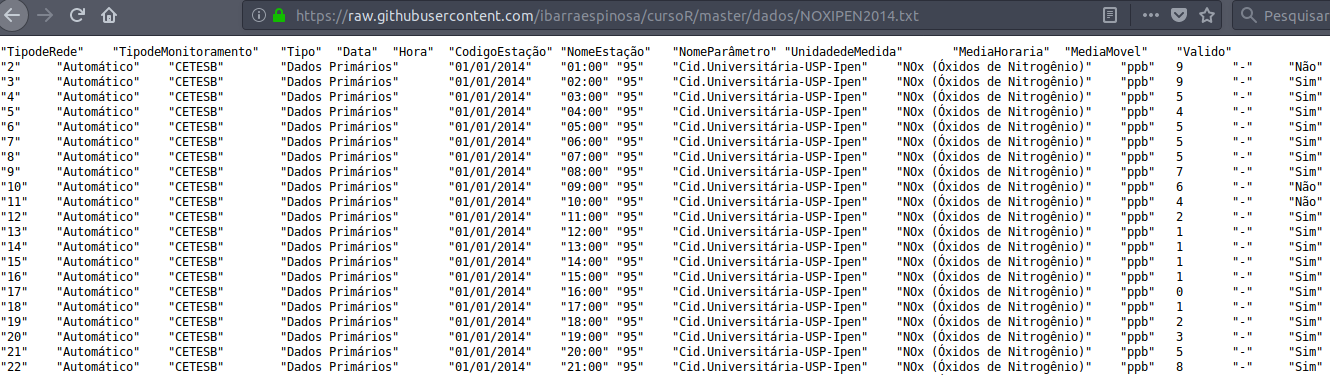
\includegraphics[width=18.47in]{figuras/f1}

O segundo arquivo é:

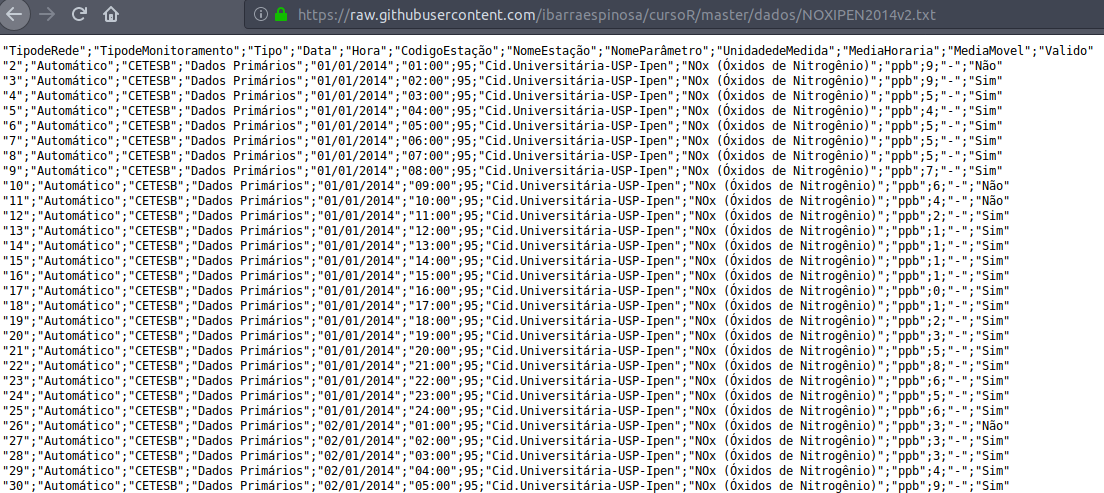
\includegraphics[width=15.33in]{figuras/f2}

qual é a diferença?

Como vemos o segundo arquivo tem separação de ``;'', entao, temos que
lero arquivo assim:

\begin{Shaded}
\begin{Highlighting}[]
\NormalTok{df2 <-}\StringTok{ }\KeywordTok{read.table}\NormalTok{(}\StringTok{"https://raw.githubusercontent.com/ibarraespinosa/cursoR/master/dados/NOXIPEN2014v2.txt"}\NormalTok{, }\DataTypeTok{sep =} \StringTok{";"}\NormalTok{)}
\KeywordTok{head}\NormalTok{(df2)}
\end{Highlighting}
\end{Shaded}

\begin{verbatim}
##   TipodeRede TipodeMonitoramento            Tipo       Data  Hora
## 2 Automático              CETESB Dados Primários 01/01/2014 01:00
## 3 Automático              CETESB Dados Primários 01/01/2014 02:00
## 4 Automático              CETESB Dados Primários 01/01/2014 03:00
## 5 Automático              CETESB Dados Primários 01/01/2014 04:00
## 6 Automático              CETESB Dados Primários 01/01/2014 05:00
## 7 Automático              CETESB Dados Primários 01/01/2014 06:00
##   CodigoEstação                NomeEstação              NomeParâmetro
## 2            95 Cid.Universitária-USP-Ipen NOx (Óxidos de Nitrogênio)
## 3            95 Cid.Universitária-USP-Ipen NOx (Óxidos de Nitrogênio)
## 4            95 Cid.Universitária-USP-Ipen NOx (Óxidos de Nitrogênio)
## 5            95 Cid.Universitária-USP-Ipen NOx (Óxidos de Nitrogênio)
## 6            95 Cid.Universitária-USP-Ipen NOx (Óxidos de Nitrogênio)
## 7            95 Cid.Universitária-USP-Ipen NOx (Óxidos de Nitrogênio)
##   UnidadedeMedida MediaHoraria MediaMovel Valido
## 2             ppb            9          -    Não
## 3             ppb            9          -    Sim
## 4             ppb            5          -    Sim
## 5             ppb            4          -    Sim
## 6             ppb            5          -    Sim
## 7             ppb            5          -    Sim
\end{verbatim}

\begin{Shaded}
\begin{Highlighting}[]
\KeywordTok{tail}\NormalTok{(df2)}
\end{Highlighting}
\end{Shaded}

\begin{verbatim}
##      TipodeRede TipodeMonitoramento            Tipo       Data  Hora
## 8577 Automático              CETESB Dados Primários 01/01/2015 19:00
## 8578 Automático              CETESB Dados Primários 01/01/2015 20:00
## 8579 Automático              CETESB Dados Primários 01/01/2015 21:00
## 8580 Automático              CETESB Dados Primários 01/01/2015 22:00
## 8581 Automático              CETESB Dados Primários 01/01/2015 23:00
## 8582 Automático              CETESB Dados Primários 01/01/2015 24:00
##      CodigoEstação                NomeEstação              NomeParâmetro
## 8577            95 Cid.Universitária-USP-Ipen NOx (Óxidos de Nitrogênio)
## 8578            95 Cid.Universitária-USP-Ipen NOx (Óxidos de Nitrogênio)
## 8579            95 Cid.Universitária-USP-Ipen NOx (Óxidos de Nitrogênio)
## 8580            95 Cid.Universitária-USP-Ipen NOx (Óxidos de Nitrogênio)
## 8581            95 Cid.Universitária-USP-Ipen NOx (Óxidos de Nitrogênio)
## 8582            95 Cid.Universitária-USP-Ipen NOx (Óxidos de Nitrogênio)
##      UnidadedeMedida MediaHoraria MediaMovel Valido
## 8577             ppb            3          -    Sim
## 8578             ppb            8          -    Sim
## 8579             ppb           11          -    Sim
## 8580             ppb           11          -    Sim
## 8581             ppb           16          -    Sim
## 8582             ppb           NA          -    Sim
\end{verbatim}

\subsection{Qua dificultades tu já enfrentou importando
dados?}\label{qua-dificultades-tu-ja-enfrentou-importando-dados}

\section{Processando nossa
data-frame}\label{processando-nossa-data-frame}

Tem numeroas formas e pacotes para ordenar, arrangiar (Arrange), mutar e
cambiar as data-frames. As mais conhecidas são provablemente do universe
\emph{tidyverse} com o famoso pacote \emph{dplyr}. Mas, nesta curso
vamos focar em \textbf{base}.

Vamos então revisar a classe de cada columna do nosso data-frame com a
função \texttt{sapply}, apresentada em outro capitulo, mas se quiser, da
uma olhada em \texttt{?sapply}.

\begin{Shaded}
\begin{Highlighting}[]
\KeywordTok{sapply}\NormalTok{(df, class)}
\end{Highlighting}
\end{Shaded}

\begin{verbatim}
##          TipodeRede TipodeMonitoramento                Tipo 
##            "factor"            "factor"            "factor" 
##                Data                Hora       CodigoEstação 
##            "factor"            "factor"           "integer" 
##         NomeEstação       NomeParâmetro     UnidadedeMedida 
##            "factor"            "factor"            "factor" 
##        MediaHoraria          MediaMovel              Valido 
##           "integer"            "factor"            "factor"
\end{verbatim}

Quando nos trabalhamos com series de tempo, é importante ter a variabel
de tempo reconhecida como ``tempo'', especificamente como classe
``POSIXct''. Mas, a classe de Data é ``factor'' e de Hora tambem
``factor'', o que é ruim. Então, vamos criar uma variabel de tempo mais
standard com formato 2018-04-30 18:32:01.

Para isso temos que grudar as variabel Data e Hora. Faremios isso numa
nova varaibel chamada tempo\_char, adicionando ela diretamente no
\texttt{df} com o cifrão DOLLAR \$. O grude pode ser feito com as
funções \texttt{paste} ou \texttt{paste0}.

\begin{Shaded}
\begin{Highlighting}[]
\NormalTok{df}\OperatorTok{$}\NormalTok{tempo_char <-}\StringTok{ }\KeywordTok{paste}\NormalTok{(df}\OperatorTok{$}\NormalTok{Data, df}\OperatorTok{$}\NormalTok{Hora)}
\KeywordTok{head}\NormalTok{(df}\OperatorTok{$}\NormalTok{tempo_char)}
\end{Highlighting}
\end{Shaded}

\begin{verbatim}
## [1] "01/01/2014 01:00" "01/01/2014 02:00" "01/01/2014 03:00"
## [4] "01/01/2014 04:00" "01/01/2014 05:00" "01/01/2014 06:00"
\end{verbatim}

\begin{Shaded}
\begin{Highlighting}[]
\KeywordTok{class}\NormalTok{(df}\OperatorTok{$}\NormalTok{tempo_char)}
\end{Highlighting}
\end{Shaded}

\begin{verbatim}
## [1] "character"
\end{verbatim}

Esta melhorando mas ainda tem clase character.

Para convertir a nossa classe POSIXct podemos usar a função
\texttt{as.POSIXct} (olha \texttt{as.POSIXct}). Seus argumentos são:

\begin{Shaded}
\begin{Highlighting}[]
\KeywordTok{args}\NormalTok{(as.POSIXct)}
\end{Highlighting}
\end{Shaded}

\begin{verbatim}
## function (x, tz = "", ...) 
## NULL
\end{verbatim}

Então, vamos criar outra variabel tempo o formato POSIXct

\begin{Shaded}
\begin{Highlighting}[]
\NormalTok{df}\OperatorTok{$}\NormalTok{tempo <-}\StringTok{ }\KeywordTok{as.POSIXct}\NormalTok{(}\DataTypeTok{x =}\NormalTok{ df}\OperatorTok{$}\NormalTok{tempo_char, }\DataTypeTok{tz =} \StringTok{"Americas/Sao_Paulo"}\NormalTok{, }
                       \DataTypeTok{format =} \StringTok{"%d/%m/%Y %H:%M"}\NormalTok{)}
\KeywordTok{head}\NormalTok{(df}\OperatorTok{$}\NormalTok{tempo)}
\end{Highlighting}
\end{Shaded}

\begin{verbatim}
## [1] "2014-01-01 01:00:00 Americas" "2014-01-01 02:00:00 Americas"
## [3] "2014-01-01 03:00:00 Americas" "2014-01-01 04:00:00 Americas"
## [5] "2014-01-01 05:00:00 Americas" "2014-01-01 06:00:00 Americas"
\end{verbatim}

\begin{Shaded}
\begin{Highlighting}[]
\KeywordTok{class}\NormalTok{(df}\OperatorTok{$}\NormalTok{tempo)}
\end{Highlighting}
\end{Shaded}

\begin{verbatim}
## [1] "POSIXct" "POSIXt"
\end{verbatim}

Agora, vamos a extraer os dias da semana do tempo, mes e dia juliano:

\begin{Shaded}
\begin{Highlighting}[]
\NormalTok{df}\OperatorTok{$}\NormalTok{weekdays <-}\StringTok{ }\KeywordTok{weekdays}\NormalTok{(df}\OperatorTok{$}\NormalTok{tempo)}
\KeywordTok{head}\NormalTok{(df}\OperatorTok{$}\NormalTok{weekdays)}
\end{Highlighting}
\end{Shaded}

\begin{verbatim}
## [1] "quarta" "quarta" "quarta" "quarta" "quarta" "quarta"
\end{verbatim}

\begin{Shaded}
\begin{Highlighting}[]
\NormalTok{df}\OperatorTok{$}\NormalTok{mes <-}\StringTok{ }\KeywordTok{months}\NormalTok{(df}\OperatorTok{$}\NormalTok{tempo)}
\KeywordTok{head}\NormalTok{(df}\OperatorTok{$}\NormalTok{mes)}
\end{Highlighting}
\end{Shaded}

\begin{verbatim}
## [1] "janeiro" "janeiro" "janeiro" "janeiro" "janeiro" "janeiro"
\end{verbatim}

\begin{Shaded}
\begin{Highlighting}[]
\NormalTok{df}\OperatorTok{$}\NormalTok{diajuliano <-}\StringTok{ }\KeywordTok{julian}\NormalTok{(df}\OperatorTok{$}\NormalTok{tempo)}
\KeywordTok{head}\NormalTok{(df}\OperatorTok{$}\NormalTok{diajuliano)}
\end{Highlighting}
\end{Shaded}

\begin{verbatim}
## Time differences in days
## [1] 16071.04 16071.08 16071.12 16071.17 16071.21 16071.25
\end{verbatim}

\section{aggregate}\label{aggregate}

\section{subset}\label{subset}

\section{data.table, read\_xl e mais}\label{data.table-read_xl-e-mais}

data.table é um pacote que apresenta a classe \texttt{data.table}, que é
como uma versão melhorada da classe \texttt{data-frame} O termo
especifico é que \texttt{data-table} tem herencia (inherits) da classe
\texttt{data.frame}

Vamos ver como funciona data.table lendo o dois arquivos e comparar
quanto tempo demoram cada um.

\begin{Shaded}
\begin{Highlighting}[]
\NormalTok{df1 <-}\StringTok{ }\KeywordTok{print}\NormalTok{(}\KeywordTok{system.time}\NormalTok{(}\KeywordTok{read.table}\NormalTok{(}\StringTok{"https://raw.githubusercontent.com/ibarraespinosa/cursoR/master/dados/NOXIPEN2014.txt"}\NormalTok{, }\DataTypeTok{h =}\NormalTok{ T)))}
\end{Highlighting}
\end{Shaded}

\begin{verbatim}
##    user  system elapsed 
##   0.207   0.011   1.222
\end{verbatim}

\begin{Shaded}
\begin{Highlighting}[]
\KeywordTok{library}\NormalTok{(data.table)}
\NormalTok{df2 <-}\StringTok{ }\KeywordTok{print}\NormalTok{(}\KeywordTok{system.time}\NormalTok{(}\KeywordTok{fread}\NormalTok{(}\StringTok{"https://raw.githubusercontent.com/ibarraespinosa/cursoR/master/dados/NOXIPEN2014.txt"}\NormalTok{, }\DataTypeTok{h =}\NormalTok{ T)))}
\end{Highlighting}
\end{Shaded}

\begin{verbatim}
## Warning in fread("https://raw.githubusercontent.com/ibarraespinosa/
## cursoR/master/dados/NOXIPEN2014.txt", : Starting data input on line 2
## and discarding line 1 because it has too few or too many items to be
## column names or data: "TipodeRede" "TipodeMonitoramento" "Tipo" "Data"
## "Hora" "CodigoEstação" "NomeEstação" "NomeParâmetro" "UnidadedeMedida"
## "MediaHoraria" "MediaMovel" "Valido"
\end{verbatim}

\begin{verbatim}
##    user  system elapsed 
##   0.025   0.004   0.089
\end{verbatim}

olha que estamos usando a função \texttt{fread}.

read\_xl é mais uma função do universo tidyverse que permite importar
excel no R, diretamente e inteligentemente.

\section{NetCDF}\label{netcdf}

O NetCDF (Network Common Data Form) é um conjunto de bibliotecas de
software e formatos de dados independentes de máquina e autodescritivos
com suporte para criação, acesso e compartilhamento de dados científicos
orientados a matrizes. Arquivos NetCDF (criado por essa biblioteca ou
por programas que utilizam essa biblioteca) são arquivos com dados,
atributos e metadados.

O pacote \texttt{ncdf4} podes ser usado com o R para ler e escrever
estes arquivos, os comandos abaixo instalam e carregam o pacote:

\begin{Shaded}
\begin{Highlighting}[]
\KeywordTok{install.packages}\NormalTok{(}\StringTok{"ncdf4"}\NormalTok{)}
\KeywordTok{nc_version}\NormalTok{() }\CommentTok{# que retorna a versão da biblioteca que o R está utilizando}
\end{Highlighting}
\end{Shaded}

Um arquivo então pode ser ascessado por:

\begin{Shaded}
\begin{Highlighting}[]
\KeywordTok{library}\NormalTok{(}\StringTok{"ncdf4"}\NormalTok{)}
\KeywordTok{download.file}\NormalTok{(}\StringTok{"https://github.com/ibarraespinosa/cursoR/raw/master/dados/met_em.d03.2016-01-10.nc"}\NormalTok{, }\DataTypeTok{destfile =} \StringTok{"~/met_em.d03.2016-01-10.nc"}\NormalTok{)}
\NormalTok{wrf <-}\StringTok{ }\KeywordTok{nc_open}\NormalTok{(}\StringTok{"dados/met_em.d03.2016-01-10.nc"}\NormalTok{)}
\end{Highlighting}
\end{Shaded}

A partir de agora o objeto wrf, contem algumas informações sobre o
arquivo, por exemplo um \texttt{print(wrf)} ou simplesmente \texttt{wrf}
mostra o conteúdo do arquivo:

\begin{Shaded}
\begin{Highlighting}[]
\NormalTok{wrf}
\end{Highlighting}
\end{Shaded}

\begin{verbatim}
## File dados/met_em.d03.2016-01-10.nc (NC_FORMAT_64BIT):
## 
##      92 variables (excluding dimension variables):
##         char Times[DateStrLen,Time]   
##         float PRES[west_east,south_north,num_metgrid_levels,Time]   
##             FieldType: 104
##             MemoryOrder: XYZ
##             units: 
##             description: 
##             stagger: M
##             sr_x: 1
##             sr_y: 1
##         float SOIL_LAYERS[west_east,south_north,num_st_layers,Time]   
##             FieldType: 104
##             MemoryOrder: XYZ
##             units: 
##             description: 
##             stagger: M
##             sr_x: 1
##             sr_y: 1
##         float SM[west_east,south_north,num_sm_layers,Time]   
##             FieldType: 104
##             MemoryOrder: XYZ
##             units: 
##             description: 
##             stagger: M
##             sr_x: 1
##             sr_y: 1
##         float ST[west_east,south_north,num_st_layers,Time]   
##             FieldType: 104
##             MemoryOrder: XYZ
##             units: 
##             description: 
##             stagger: M
##             sr_x: 1
##             sr_y: 1
##         float GHT[west_east,south_north,num_metgrid_levels,Time]   
##             FieldType: 104
##             MemoryOrder: XYZ
##             units: m
##             description: Height
##             stagger: M
##             sr_x: 1
##             sr_y: 1
##         float HGTTROP[west_east,south_north,Time]   
##             FieldType: 104
##             MemoryOrder: XY 
##             units: m
##             description: Height of tropopause
##             stagger: M
##             sr_x: 1
##             sr_y: 1
##         float TTROP[west_east,south_north,Time]   
##             FieldType: 104
##             MemoryOrder: XY 
##             units: K
##             description: Temperature at tropopause
##             stagger: M
##             sr_x: 1
##             sr_y: 1
##         float PTROPNN[west_east,south_north,Time]   
##             FieldType: 104
##             MemoryOrder: XY 
##             units: Pa
##             description: PTROP, used for nearest neighbor interp
##             stagger: M
##             sr_x: 1
##             sr_y: 1
##         float PTROP[west_east,south_north,Time]   
##             FieldType: 104
##             MemoryOrder: XY 
##             units: Pa
##             description: Pressure of tropopause
##             stagger: M
##             sr_x: 1
##             sr_y: 1
##         float VTROP[west_east,south_north_stag,Time]   
##             FieldType: 104
##             MemoryOrder: XY 
##             units: m s-1
##             description: V                 at tropopause
##             stagger: V
##             sr_x: 1
##             sr_y: 1
##         float UTROP[west_east_stag,south_north,Time]   
##             FieldType: 104
##             MemoryOrder: XY 
##             units: m s-1
##             description: U                 at tropopause
##             stagger: U
##             sr_x: 1
##             sr_y: 1
##         float HGTMAXW[west_east,south_north,Time]   
##             FieldType: 104
##             MemoryOrder: XY 
##             units: m
##             description: Height of max wind level
##             stagger: M
##             sr_x: 1
##             sr_y: 1
##         float TMAXW[west_east,south_north,Time]   
##             FieldType: 104
##             MemoryOrder: XY 
##             units: K
##             description: Temperature at max wind level
##             stagger: M
##             sr_x: 1
##             sr_y: 1
##         float PMAXWNN[west_east,south_north,Time]   
##             FieldType: 104
##             MemoryOrder: XY 
##             units: Pa
##             description: PMAXW, used for nearest neighbor interp
##             stagger: M
##             sr_x: 1
##             sr_y: 1
##         float PMAXW[west_east,south_north,Time]   
##             FieldType: 104
##             MemoryOrder: XY 
##             units: Pa
##             description: Pressure of max wind level
##             stagger: M
##             sr_x: 1
##             sr_y: 1
##         float VMAXW[west_east,south_north_stag,Time]   
##             FieldType: 104
##             MemoryOrder: XY 
##             units: m s-1
##             description: V                 at max wind
##             stagger: V
##             sr_x: 1
##             sr_y: 1
##         float UMAXW[west_east_stag,south_north,Time]   
##             FieldType: 104
##             MemoryOrder: XY 
##             units: m s-1
##             description: U                 at max wind
##             stagger: U
##             sr_x: 1
##             sr_y: 1
##         float SNOWH[west_east,south_north,Time]   
##             FieldType: 104
##             MemoryOrder: XY 
##             units: m
##             description: Physical Snow Depth
##             stagger: M
##             sr_x: 1
##             sr_y: 1
##         float SNOW[west_east,south_north,Time]   
##             FieldType: 104
##             MemoryOrder: XY 
##             units: kg m-2
##             description: Water equivalent snow depth
##             stagger: M
##             sr_x: 1
##             sr_y: 1
##         float SKINTEMP[west_east,south_north,Time]   
##             FieldType: 104
##             MemoryOrder: XY 
##             units: K
##             description: Skin temperature
##             stagger: M
##             sr_x: 1
##             sr_y: 1
##         float SOILHGT[west_east,south_north,Time]   
##             FieldType: 104
##             MemoryOrder: XY 
##             units: m
##             description: Terrain field of source analysis
##             stagger: M
##             sr_x: 1
##             sr_y: 1
##         float LANDSEA[west_east,south_north,Time]   
##             FieldType: 104
##             MemoryOrder: XY 
##             units: proprtn
##             description: Land/Sea flag (1=land, 0 or 2=sea)
##             stagger: M
##             sr_x: 1
##             sr_y: 1
##         float SEAICE[west_east,south_north,Time]   
##             FieldType: 104
##             MemoryOrder: XY 
##             units: proprtn
##             description: Ice flag
##             stagger: M
##             sr_x: 1
##             sr_y: 1
##         float ST100200[west_east,south_north,Time]   
##             FieldType: 104
##             MemoryOrder: XY 
##             units: K
##             description: T 100-200 cm below ground layer (Bottom)
##             stagger: M
##             sr_x: 1
##             sr_y: 1
##         float ST040100[west_east,south_north,Time]   
##             FieldType: 104
##             MemoryOrder: XY 
##             units: K
##             description: T 40-100 cm below ground layer (Upper)
##             stagger: M
##             sr_x: 1
##             sr_y: 1
##         float ST010040[west_east,south_north,Time]   
##             FieldType: 104
##             MemoryOrder: XY 
##             units: K
##             description: T 10-40 cm below ground layer (Upper)
##             stagger: M
##             sr_x: 1
##             sr_y: 1
##         float ST000010[west_east,south_north,Time]   
##             FieldType: 104
##             MemoryOrder: XY 
##             units: K
##             description: T 0-10 cm below ground layer (Upper)
##             stagger: M
##             sr_x: 1
##             sr_y: 1
##         float SM100200[west_east,south_north,Time]   
##             FieldType: 104
##             MemoryOrder: XY 
##             units: fraction
##             description: Soil Moist 100-200 cm below gr layer
##             stagger: M
##             sr_x: 1
##             sr_y: 1
##         float SM040100[west_east,south_north,Time]   
##             FieldType: 104
##             MemoryOrder: XY 
##             units: fraction
##             description: Soil Moist 40-100 cm below grn layer
##             stagger: M
##             sr_x: 1
##             sr_y: 1
##         float SM010040[west_east,south_north,Time]   
##             FieldType: 104
##             MemoryOrder: XY 
##             units: fraction
##             description: Soil Moist 10-40 cm below grn layer
##             stagger: M
##             sr_x: 1
##             sr_y: 1
##         float SM000010[west_east,south_north,Time]   
##             FieldType: 104
##             MemoryOrder: XY 
##             units: fraction
##             description: Soil Moist 0-10 cm below grn layer (Up)
##             stagger: M
##             sr_x: 1
##             sr_y: 1
##         float PSFC[west_east,south_north,Time]   
##             FieldType: 104
##             MemoryOrder: XY 
##             units: Pa
##             description: Surface Pressure
##             stagger: M
##             sr_x: 1
##             sr_y: 1
##         float RH[west_east,south_north,num_metgrid_levels,Time]   
##             FieldType: 104
##             MemoryOrder: XYZ
##             units: %
##             description: Relative Humidity
##             stagger: M
##             sr_x: 1
##             sr_y: 1
##         float VV[west_east,south_north_stag,num_metgrid_levels,Time]   
##             FieldType: 104
##             MemoryOrder: XYZ
##             units: m s-1
##             description: V
##             stagger: V
##             sr_x: 1
##             sr_y: 1
##         float UU[west_east_stag,south_north,num_metgrid_levels,Time]   
##             FieldType: 104
##             MemoryOrder: XYZ
##             units: m s-1
##             description: U
##             stagger: U
##             sr_x: 1
##             sr_y: 1
##         float TT[west_east,south_north,num_metgrid_levels,Time]   
##             FieldType: 104
##             MemoryOrder: XYZ
##             units: K
##             description: Temperature
##             stagger: M
##             sr_x: 1
##             sr_y: 1
##         float PMSL[west_east,south_north,Time]   
##             FieldType: 104
##             MemoryOrder: XY 
##             units: Pa
##             description: Sea-level Pressure
##             stagger: M
##             sr_x: 1
##             sr_y: 1
##         float URB_PARAM[west_east,south_north,z-dimension0132,Time]   
##             FieldType: 104
##             MemoryOrder: XYZ
##             units: dimensionless
##             description: Urban_Parameters
##             stagger: M
##             sr_x: 1
##             sr_y: 1
##         float LAKE_DEPTH[west_east,south_north,Time]   
##             FieldType: 104
##             MemoryOrder: XY 
##             units: meters MSL
##             description: Topography height
##             stagger: M
##             sr_x: 1
##             sr_y: 1
##         float VAR_SSO[west_east,south_north,Time]   
##             FieldType: 104
##             MemoryOrder: XY 
##             units: meters2 MSL
##             description: Variance of Subgrid Scale Orography
##             stagger: M
##             sr_x: 1
##             sr_y: 1
##         float OL4[west_east,south_north,Time]   
##             FieldType: 104
##             MemoryOrder: XY 
##             units: whoknows
##             description: something
##             stagger: M
##             sr_x: 1
##             sr_y: 1
##         float OL3[west_east,south_north,Time]   
##             FieldType: 104
##             MemoryOrder: XY 
##             units: whoknows
##             description: something
##             stagger: M
##             sr_x: 1
##             sr_y: 1
##         float OL2[west_east,south_north,Time]   
##             FieldType: 104
##             MemoryOrder: XY 
##             units: whoknows
##             description: something
##             stagger: M
##             sr_x: 1
##             sr_y: 1
##         float OL1[west_east,south_north,Time]   
##             FieldType: 104
##             MemoryOrder: XY 
##             units: whoknows
##             description: something
##             stagger: M
##             sr_x: 1
##             sr_y: 1
##         float OA4[west_east,south_north,Time]   
##             FieldType: 104
##             MemoryOrder: XY 
##             units: whoknows
##             description: something
##             stagger: M
##             sr_x: 1
##             sr_y: 1
##         float OA3[west_east,south_north,Time]   
##             FieldType: 104
##             MemoryOrder: XY 
##             units: whoknows
##             description: something
##             stagger: M
##             sr_x: 1
##             sr_y: 1
##         float OA2[west_east,south_north,Time]   
##             FieldType: 104
##             MemoryOrder: XY 
##             units: whoknows
##             description: something
##             stagger: M
##             sr_x: 1
##             sr_y: 1
##         float OA1[west_east,south_north,Time]   
##             FieldType: 104
##             MemoryOrder: XY 
##             units: whoknows
##             description: something
##             stagger: M
##             sr_x: 1
##             sr_y: 1
##         float VAR[west_east,south_north,Time]   
##             FieldType: 104
##             MemoryOrder: XY 
##             units: whoknows
##             description: something
##             stagger: M
##             sr_x: 1
##             sr_y: 1
##         float CON[west_east,south_north,Time]   
##             FieldType: 104
##             MemoryOrder: XY 
##             units: whoknows
##             description: something
##             stagger: M
##             sr_x: 1
##             sr_y: 1
##         float SLOPECAT[west_east,south_north,Time]   
##             FieldType: 104
##             MemoryOrder: XY 
##             units: category
##             description: Dominant category
##             stagger: M
##             sr_x: 1
##             sr_y: 1
##         float SNOALB[west_east,south_north,Time]   
##             FieldType: 104
##             MemoryOrder: XY 
##             units: percent
##             description: Maximum snow albedo
##             stagger: M
##             sr_x: 1
##             sr_y: 1
##         float LAI12M[west_east,south_north,z-dimension0012,Time]   
##             FieldType: 104
##             MemoryOrder: XYZ
##             units: m^2/m^2
##             description: MODIS LAI
##             stagger: M
##             sr_x: 1
##             sr_y: 1
##         float GREENFRAC[west_east,south_north,z-dimension0012,Time]   
##             FieldType: 104
##             MemoryOrder: XYZ
##             units: fraction
##             description: MODIS FPAR
##             stagger: M
##             sr_x: 1
##             sr_y: 1
##         float ALBEDO12M[west_east,south_north,z-dimension0012,Time]   
##             FieldType: 104
##             MemoryOrder: XYZ
##             units: percent
##             description: Monthly surface albedo
##             stagger: M
##             sr_x: 1
##             sr_y: 1
##         float SCB_DOM[west_east,south_north,Time]   
##             FieldType: 104
##             MemoryOrder: XY 
##             units: category
##             description: Dominant category
##             stagger: M
##             sr_x: 1
##             sr_y: 1
##         float SOILCBOT[west_east,south_north,z-dimension0016,Time]   
##             FieldType: 104
##             MemoryOrder: XYZ
##             units: category
##             description: 16-category bottom-layer soil type
##             stagger: M
##             sr_x: 1
##             sr_y: 1
##         float SCT_DOM[west_east,south_north,Time]   
##             FieldType: 104
##             MemoryOrder: XY 
##             units: category
##             description: Dominant category
##             stagger: M
##             sr_x: 1
##             sr_y: 1
##         float SOILCTOP[west_east,south_north,z-dimension0016,Time]   
##             FieldType: 104
##             MemoryOrder: XYZ
##             units: category
##             description: 16-category top-layer soil type
##             stagger: M
##             sr_x: 1
##             sr_y: 1
##         float SOILTEMP[west_east,south_north,Time]   
##             FieldType: 104
##             MemoryOrder: XY 
##             units: Kelvin
##             description: Annual mean deep soil temperature
##             stagger: M
##             sr_x: 1
##             sr_y: 1
##         float HGT_M[west_east,south_north,Time]   
##             FieldType: 104
##             MemoryOrder: XY 
##             units: meters MSL
##             description: GMTED2010 30-arc-second topography height
##             stagger: M
##             sr_x: 1
##             sr_y: 1
##         float LU_INDEX[west_east,south_north,Time]   
##             FieldType: 104
##             MemoryOrder: XY 
##             units: category
##             description: Dominant category
##             stagger: M
##             sr_x: 1
##             sr_y: 1
##         float LANDUSEF[west_east,south_north,z-dimension0024,Time]   
##             FieldType: 104
##             MemoryOrder: XYZ
##             units: category
##             description: 24-category USGS landuse
##             stagger: M
##             sr_x: 1
##             sr_y: 1
##         float COSALPHA_V[west_east,south_north_stag,Time]   
##             FieldType: 104
##             MemoryOrder: XY 
##             units: none
##             description: Cosine of rotation angle on V grid
##             stagger: V
##             sr_x: 1
##             sr_y: 1
##         float SINALPHA_V[west_east,south_north_stag,Time]   
##             FieldType: 104
##             MemoryOrder: XY 
##             units: none
##             description: Sine of rotation angle on V grid
##             stagger: V
##             sr_x: 1
##             sr_y: 1
##         float COSALPHA_U[west_east_stag,south_north,Time]   
##             FieldType: 104
##             MemoryOrder: XY 
##             units: none
##             description: Cosine of rotation angle on U grid
##             stagger: U
##             sr_x: 1
##             sr_y: 1
##         float SINALPHA_U[west_east_stag,south_north,Time]   
##             FieldType: 104
##             MemoryOrder: XY 
##             units: none
##             description: Sine of rotation angle on U grid
##             stagger: U
##             sr_x: 1
##             sr_y: 1
##         float XLONG_C[west_east_stag,south_north_stag,Time]   
##             FieldType: 104
##             MemoryOrder: XY 
##             units: degrees longitude
##             description: Longitude at grid cell corners
##             stagger: CORNER
##             sr_x: 1
##             sr_y: 1
##         float XLAT_C[west_east_stag,south_north_stag,Time]   
##             FieldType: 104
##             MemoryOrder: XY 
##             units: degrees latitude
##             description: Latitude at grid cell corners
##             stagger: CORNER
##             sr_x: 1
##             sr_y: 1
##         float LANDMASK[west_east,south_north,Time]   
##             FieldType: 104
##             MemoryOrder: XY 
##             units: none
##             description: Landmask : 1=land, 0=water
##             stagger: M
##             sr_x: 1
##             sr_y: 1
##         float COSALPHA[west_east,south_north,Time]   
##             FieldType: 104
##             MemoryOrder: XY 
##             units: none
##             description: Cosine of rotation angle
##             stagger: M
##             sr_x: 1
##             sr_y: 1
##         float SINALPHA[west_east,south_north,Time]   
##             FieldType: 104
##             MemoryOrder: XY 
##             units: none
##             description: Sine of rotation angle
##             stagger: M
##             sr_x: 1
##             sr_y: 1
##         float F[west_east,south_north,Time]   
##             FieldType: 104
##             MemoryOrder: XY 
##             units: -
##             description: Coriolis F parameter
##             stagger: M
##             sr_x: 1
##             sr_y: 1
##         float E[west_east,south_north,Time]   
##             FieldType: 104
##             MemoryOrder: XY 
##             units: -
##             description: Coriolis E parameter
##             stagger: M
##             sr_x: 1
##             sr_y: 1
##         float MAPFAC_UY[west_east_stag,south_north,Time]   
##             FieldType: 104
##             MemoryOrder: XY 
##             units: none
##             description: Mapfactor (y-dir) on U grid
##             stagger: U
##             sr_x: 1
##             sr_y: 1
##         float MAPFAC_VY[west_east,south_north_stag,Time]   
##             FieldType: 104
##             MemoryOrder: XY 
##             units: none
##             description: Mapfactor (y-dir) on V grid
##             stagger: V
##             sr_x: 1
##             sr_y: 1
##         float MAPFAC_MY[west_east,south_north,Time]   
##             FieldType: 104
##             MemoryOrder: XY 
##             units: none
##             description: Mapfactor (y-dir) on mass grid
##             stagger: M
##             sr_x: 1
##             sr_y: 1
##         float MAPFAC_UX[west_east_stag,south_north,Time]   
##             FieldType: 104
##             MemoryOrder: XY 
##             units: none
##             description: Mapfactor (x-dir) on U grid
##             stagger: U
##             sr_x: 1
##             sr_y: 1
##         float MAPFAC_VX[west_east,south_north_stag,Time]   
##             FieldType: 104
##             MemoryOrder: XY 
##             units: none
##             description: Mapfactor (x-dir) on V grid
##             stagger: V
##             sr_x: 1
##             sr_y: 1
##         float MAPFAC_MX[west_east,south_north,Time]   
##             FieldType: 104
##             MemoryOrder: XY 
##             units: none
##             description: Mapfactor (x-dir) on mass grid
##             stagger: M
##             sr_x: 1
##             sr_y: 1
##         float MAPFAC_U[west_east_stag,south_north,Time]   
##             FieldType: 104
##             MemoryOrder: XY 
##             units: none
##             description: Mapfactor on U grid
##             stagger: U
##             sr_x: 1
##             sr_y: 1
##         float MAPFAC_V[west_east,south_north_stag,Time]   
##             FieldType: 104
##             MemoryOrder: XY 
##             units: none
##             description: Mapfactor on V grid
##             stagger: V
##             sr_x: 1
##             sr_y: 1
##         float MAPFAC_M[west_east,south_north,Time]   
##             FieldType: 104
##             MemoryOrder: XY 
##             units: none
##             description: Mapfactor on mass grid
##             stagger: M
##             sr_x: 1
##             sr_y: 1
##         float CLONG[west_east,south_north,Time]   
##             FieldType: 104
##             MemoryOrder: XY 
##             units: degrees longitude
##             description: Computational longitude on mass grid
##             stagger: M
##             sr_x: 1
##             sr_y: 1
##         float CLAT[west_east,south_north,Time]   
##             FieldType: 104
##             MemoryOrder: XY 
##             units: degrees latitude
##             description: Computational latitude on mass grid
##             stagger: M
##             sr_x: 1
##             sr_y: 1
##         float XLONG_U[west_east_stag,south_north,Time]   
##             FieldType: 104
##             MemoryOrder: XY 
##             units: degrees longitude
##             description: Longitude on U grid
##             stagger: U
##             sr_x: 1
##             sr_y: 1
##         float XLAT_U[west_east_stag,south_north,Time]   
##             FieldType: 104
##             MemoryOrder: XY 
##             units: degrees latitude
##             description: Latitude on U grid
##             stagger: U
##             sr_x: 1
##             sr_y: 1
##         float XLONG_V[west_east,south_north_stag,Time]   
##             FieldType: 104
##             MemoryOrder: XY 
##             units: degrees longitude
##             description: Longitude on V grid
##             stagger: V
##             sr_x: 1
##             sr_y: 1
##         float XLAT_V[west_east,south_north_stag,Time]   
##             FieldType: 104
##             MemoryOrder: XY 
##             units: degrees latitude
##             description: Latitude on V grid
##             stagger: V
##             sr_x: 1
##             sr_y: 1
##         float XLONG_M[west_east,south_north,Time]   
##             FieldType: 104
##             MemoryOrder: XY 
##             units: degrees longitude
##             description: Longitude on mass grid
##             stagger: M
##             sr_x: 1
##             sr_y: 1
##         float XLAT_M[west_east,south_north,Time]   
##             FieldType: 104
##             MemoryOrder: XY 
##             units: degrees latitude
##             description: Latitude on mass grid
##             stagger: M
##             sr_x: 1
##             sr_y: 1
## 
##      13 dimensions:
##         Time  Size:1   *** is unlimited ***
##         DateStrLen  Size:19
##         west_east  Size:51
##         south_north  Size:51
##         num_metgrid_levels  Size:27
##         num_st_layers  Size:4
##         num_sm_layers  Size:4
##         south_north_stag  Size:52
##         west_east_stag  Size:52
##         z-dimension0132  Size:132
##         z-dimension0012  Size:12
##         z-dimension0016  Size:16
##         z-dimension0024  Size:24
## 
##     76 global attributes:
##         TITLE: OUTPUT FROM METGRID V3.9.1
##         SIMULATION_START_DATE: 2016-01-10_00:00:00
##         WEST-EAST_GRID_DIMENSION: 52
##         SOUTH-NORTH_GRID_DIMENSION: 52
##         BOTTOM-TOP_GRID_DIMENSION: 27
##         WEST-EAST_PATCH_START_UNSTAG: 1
##         WEST-EAST_PATCH_END_UNSTAG: 51
##         WEST-EAST_PATCH_START_STAG: 1
##         WEST-EAST_PATCH_END_STAG: 52
##         SOUTH-NORTH_PATCH_START_UNSTAG: 1
##         SOUTH-NORTH_PATCH_END_UNSTAG: 51
##         SOUTH-NORTH_PATCH_START_STAG: 1
##         SOUTH-NORTH_PATCH_END_STAG: 52
##         GRIDTYPE: C
##         DX: 1000
##         DY: 1000
##         DYN_OPT: 2
##         CEN_LAT: -23.5996932983398
##         CEN_LON: -46.6294555664062
##         TRUELAT1: -23
##         TRUELAT2: -24
##         MOAD_CEN_LAT: -23.6000061035156
##         STAND_LON: -45
##         POLE_LAT: 90
##         POLE_LON: 0
##         corner_lats: -23.8218078613281
##          corner_lats: -23.3720855712891
##          corner_lats: -23.3771743774414
##          corner_lats: -23.826904296875
##          corner_lats: -23.8217391967773
##          corner_lats: -23.3720245361328
##          corner_lats: -23.3772277832031
##          corner_lats: -23.8269424438477
##          corner_lats: -23.826286315918
##          corner_lats: -23.3675918579102
##          corner_lats: -23.372673034668
##          corner_lats: -23.8314056396484
##          corner_lats: -23.8262329101562
##          corner_lats: -23.3675231933594
##          corner_lats: -23.3727111816406
##          corner_lats: -23.8314437866211
##         corner_lons: -46.8780517578125
##          corner_lons: -46.8716430664062
##          corner_lons: -46.3817138671875
##          corner_lons: -46.3864440917969
##          corner_lons: -46.8829650878906
##          corner_lons: -46.8765258789062
##          corner_lons: -46.3768005371094
##          corner_lons: -46.3815307617188
##          corner_lons: -46.8781127929688
##          corner_lons: -46.87158203125
##          corner_lons: -46.3816528320312
##          corner_lons: -46.386474609375
##          corner_lons: -46.8830261230469
##          corner_lons: -46.87646484375
##          corner_lons: -46.3767700195312
##          corner_lons: -46.3815612792969
##         MAP_PROJ: 1
##         MMINLU: USGS
##         NUM_LAND_CAT: 24
##         ISWATER: 16
##         ISLAKE: -1
##         ISICE: 24
##         ISURBAN: 1
##         ISOILWATER: 14
##         grid_id: 3
##         parent_id: 2
##         i_parent_start: 35
##         j_parent_start: 33
##         i_parent_end: 51
##         j_parent_end: 49
##         parent_grid_ratio: 3
##         sr_x: 1
##         sr_y: 1
##         NUM_METGRID_SOIL_LEVELS: 4
##         FLAG_METGRID: 1
##         FLAG_EXCLUDED_MIDDLE: 0
##         FLAG_SOIL_LAYERS: 1
##         FLAG_SNOW: 1
##         FLAG_PSFC: 1
##         FLAG_SM000010: 1
##         FLAG_SM010040: 1
##         FLAG_SM040100: 1
##         FLAG_SM100200: 1
##         FLAG_ST000010: 1
##         FLAG_ST010040: 1
##         FLAG_ST040100: 1
##         FLAG_ST100200: 1
##         FLAG_SLP: 1
##         FLAG_SNOWH: 1
##         FLAG_SOILHGT: 1
##         FLAG_UTROP: 1
##         FLAG_VTROP: 1
##         FLAG_TTROP: 1
##         FLAG_PTROP: 1
##         FLAG_PTROPNN: 1
##         FLAG_HGTTROP: 1
##         FLAG_UMAXW: 1
##         FLAG_VMAXW: 1
##         FLAG_TMAXW: 1
##         FLAG_PMAXW: 1
##         FLAG_PMAXWNN: 1
##         FLAG_HGTMAXW: 1
##         FLAG_MF_XY: 1
##         FLAG_LAI12M: 1
##         FLAG_LAKE_DEPTH: 1
\end{verbatim}

Entre a informação mostrada na tela estão o nome do arquivo (e versão da
biblioteca usada para criar), numero de variáveis (92 no arquivo de
exemplo), uma descrição de cada variavel (incluindo atributos) as
dimenções (13 para esse aquivo) e os atributos globais.

Agora vamos abrir alguma variável:

\begin{Shaded}
\begin{Highlighting}[]
\KeywordTok{names}\NormalTok{(wrf}\OperatorTok{$}\NormalTok{var)              }\CommentTok{# print no nome de cada variavel}
\end{Highlighting}
\end{Shaded}

\begin{verbatim}
##  [1] "Times"       "PRES"        "SOIL_LAYERS" "SM"          "ST"         
##  [6] "GHT"         "HGTTROP"     "TTROP"       "PTROPNN"     "PTROP"      
## [11] "VTROP"       "UTROP"       "HGTMAXW"     "TMAXW"       "PMAXWNN"    
## [16] "PMAXW"       "VMAXW"       "UMAXW"       "SNOWH"       "SNOW"       
## [21] "SKINTEMP"    "SOILHGT"     "LANDSEA"     "SEAICE"      "ST100200"   
## [26] "ST040100"    "ST010040"    "ST000010"    "SM100200"    "SM040100"   
## [31] "SM010040"    "SM000010"    "PSFC"        "RH"          "VV"         
## [36] "UU"          "TT"          "PMSL"        "URB_PARAM"   "LAKE_DEPTH" 
## [41] "VAR_SSO"     "OL4"         "OL3"         "OL2"         "OL1"        
## [46] "OA4"         "OA3"         "OA2"         "OA1"         "VAR"        
## [51] "CON"         "SLOPECAT"    "SNOALB"      "LAI12M"      "GREENFRAC"  
## [56] "ALBEDO12M"   "SCB_DOM"     "SOILCBOT"    "SCT_DOM"     "SOILCTOP"   
## [61] "SOILTEMP"    "HGT_M"       "LU_INDEX"    "LANDUSEF"    "COSALPHA_V" 
## [66] "SINALPHA_V"  "COSALPHA_U"  "SINALPHA_U"  "XLONG_C"     "XLAT_C"     
## [71] "LANDMASK"    "COSALPHA"    "SINALPHA"    "F"           "E"          
## [76] "MAPFAC_UY"   "MAPFAC_VY"   "MAPFAC_MY"   "MAPFAC_UX"   "MAPFAC_VX"  
## [81] "MAPFAC_MX"   "MAPFAC_U"    "MAPFAC_V"    "MAPFAC_M"    "CLONG"      
## [86] "CLAT"        "XLONG_U"     "XLAT_U"      "XLONG_V"     "XLAT_V"     
## [91] "XLONG_M"     "XLAT_M"
\end{verbatim}

\begin{Shaded}
\begin{Highlighting}[]
\NormalTok{ST <-}\StringTok{ }\KeywordTok{ncvar_get}\NormalTok{(wrf, }\StringTok{"ST"}\NormalTok{)  }\CommentTok{# escolho você picachu}
\end{Highlighting}
\end{Shaded}

ncvar\_get Read data from a netCDF file

ncatt\_get Get attribute from netCDF file ncatt\_put Put an attribute
into a netCDF file

ncvar\_add Add New netCDF Variable to Existing File
ncvar\_change\_missval Change the Missing Value For a netCDF Variable
ncvar\_def Define a netCDF Variable ncvar\_put Write data to a netCDF
file ncvar\_rename Rename an Existing Variable in a netCDF File

nc\_version Report version of ncdf4 library nc\_create Create a netCDF
File ncdim\_def Define a netCDF Dimension nc\_enddef Takes a netCDF file
out of define mode nc\_redef Puts a netCDF file back into define mode

nc\_close Close a netCDF File nc\_sync Synchronize (flush to disk) a
netCDF File

Para salvar toda informação e liberar o ascesso ao arquivo use a função
\texttt{nc\_close} (ou a função \texttt{nc\_sync} que sincroniza o
NetCDF carregado na memória com o NetCDF no Disco)

\begin{Shaded}
\begin{Highlighting}[]
\KeywordTok{nc_close}\NormalTok{(wrf)}
\end{Highlighting}
\end{Shaded}

\section{Binarios}\label{binarios}

\chapter{Applications}\label{applications}

Some \emph{significant} applications are demonstrated in this chapter.

\section{Example one}\label{example-one}

\section{Example two}\label{example-two}

\chapter{Final Words}\label{final-words}

We have finished a nice book.

\bibliography{book.bib,packages.bib}


\end{document}
